\chapter{逻辑与博弈}\label{chap:game}

2016年3月,围棋界迎来了一场前所未有的挑战——谷歌DeepMind团队开发的人工智能 \emph{AlphaGo}\index{AlphaGo} 挑战韩国围棋九段世界冠军李世乭。这场比赛不仅引发了全球的关注,更成为了人工智能领域的里程碑。

围棋被认为是极其复杂的游戏,其复杂性远远超越国际象棋,因此,许多人曾认为围棋是人工智能无法攻克的“堡垒”。然而,AlphaGo改变了这一看法。

在首局比赛中,李世乭似乎还没有完全适应对手是一台超级计算机。起初,李世乭运用了传统的围棋策略,期待通过人类棋手的经验与直觉来击败AlphaGo。然而,比赛后期,AlphaGo展现出极其强大的计算能力,持续挖掘并利用局面中的潜在机会。最终,李世乭被逼至绝境,AlphaGo成功赢下了第一局。

第二局比赛成为整个系列赛的关键点,也正是在这一局中,AlphaGo下出了它最令人惊叹的一步——第37手。这一手棋打破了人们对围棋的传统理解,AlphaGo将白子下在了一个似乎毫无意义的位置,许多围棋专家和职业棋手一度认为这是“臭棋”。李世乭一度陷入沉思,走出赛场短暂休息。

然而,随着局面的展开,这步棋逐渐展示出了它的深远战略意图,它不仅打乱了李世乭的布局,还为AlphaGo赢得了巨大优势。最终,李世乭输掉了第二局,这一局被认为是AlphaGo表现出超越人类直觉的关键胜利。

第三局中,李世乭试图改变策略,以更加复杂、创新且进攻的方式应对AlphaGo。然而,AlphaGo表现得更加冷静和高效,它不仅成功化解了李世乭的进攻,还逐渐将局面转变为对自己有利的形式。在对局的后期,李世乭再次被迫认输。至此,AlphaGo以3:0的比分提前赢得了这场五局比赛的胜利。

尽管前面三局失利,李世乭并没有放弃。在第四局中,他展示了超凡的创造力和直觉,走出了被称为“神之一手”的第78手。这一手棋打破了AlphaGo的计算预期,突然扭转了局面,让AlphaGo陷入困境。尽管AlphaGo做出了顽强的抵抗,但李世乭凭借这一步棋最终赢得了这一局胜利。这是人类在整个比赛中唯一的一胜。

在最后一局比赛中,李世乭保持了极高的斗志,但AlphaGo通过深度学习积累的经验和计算能力再次发挥作用。尽管李世乭尽力应对,但AlphaGo在关键时刻掌控了局面,最终赢得了第五局的胜利。整个比赛以4:1的结果结束,AlphaGo取得了压倒性的胜利。

李世乭与AlphaGo的第四局对决,不仅是那一次比赛的唯一一次胜利,也是此后人类与顶尖围棋人工智能较量中的最后一次胜利。而第二局AlphaGo的神之一手,人类至今不能理解,只能效仿。AlphaGo通过学习人类棋谱,再通过自我对弈,最终超越了人类的认知,成为了围棋的新王者。

毫无疑问,这一比赛彻底的改写了围棋的历史。过去,围棋被视为一种具有智慧和创造力的艺术;但现在,围棋选手获胜唯一的出路是模仿人工智能的策略。后来,\emph{AlphaGo Zero}\index{AlphaGo Zero} 横空出世,它完全不依赖人类知识,但是完胜AlphaGo。人类积累了几千年的围棋经验,在人工智能面前显得如此渺小。

围棋代表了一种特别的决策与优化问题:我们的决策依赖于对手,而对手的决策又依赖于我们。这样的决策问题形成了\emph{博弈论}\index{博弈论}的研究对象. 博弈是如此复杂,以至于如何恰当地描述博弈的过程都是一个巨大的挑战。本章的目标是给出博弈论的通用语言和基本概念,以及一些经典的博弈模型和他们在人工智能中的应用.

\section{博弈的基本语言:以井字棋为例}\label{sec:game-basic}

大家都玩过井字棋,这是一个简单的博弈. 如\Cref{???}\lhysays{画个图} 所示,在棋局中,两名玩家轮流在一个$3\times 3$的棋盘上放置自己的标记(X或O),直到有一方连成一条线(横、竖、斜)或者棋盘填满,在前一种情况下,这个玩家获胜,否则平局. 

上面的描述是自然语言,并不能被计算机直接理解. 我们需要将这个博弈的过程形式化,以便计算机能够理解和处理. 在井字棋中,有如下的基本概念:
\begin{itemize}
    \item \emph{玩家}\index{玩家}: 两名玩家,一个执X子,另一个执O子.
    \item 棋盘\emph{局面}\index{局面}: 棋盘的当前状态,包括每个格子的占据情况(X,O或空).
    \item \emph{行动}\index{行动}: 每个玩家轮流在空格中放置自己的棋(X或O),直到出现胜负或棋盘填满.
    \item \emph{收益}\index{收益}: 游戏结束时,根据游戏的结果确定每个玩家的收益,胜者为$+1$,平局为$0$,败者为$-1$.
\end{itemize}

以上概念足够描述\emph{博弈}是什么了。然而,它不足以描述\emph{玩家}是如何下棋的。为此,我们需要引入\emph{策略}\index{策略}的概念. 我们将在本章中看到,如何定义策略是博弈论中最为复杂的问题之一。此刻,我们只关注井字棋这一场景中的策略.

我们假定玩家都有充分大的计算能力和记忆力。于是,玩家可以记住这一次游戏中所有的局面,以及每个轮次的自己和对手的行动. 玩家可以知道自己的内心活动(也就是有内省的能力),但是,玩家绝不可能知道对手的内心活动,更不知道他下一步会怎么走. 总而言之,玩家只能知道对大家都是公开的这些信息以及自己独有的信息。

在知道所有的信息之后,玩家需要决定每一轮的走法。或许他会猜测对手的心理活动以及策略,并以此为根据做出自己的决策. 他也可能完全不管对手的行动,而是我行我素。无论如何,玩家的决策都是基于他所知道的信息,因而我们可以认为玩家的决策是一个\emph{映射},将他知道的信息映射到他的行动空间。

因此,玩家的\emph{策略},就是一个\emph{映射},给定当前处于哪个轮次、所有历史局面和行动之后,它会输出下一步的行动. 

需要注意的是,每个玩家在开局的时候就要选好自己的策略,此后只能遵循这个策略进行行动。初看之下,这一定义是极强的,我们似乎无法在游戏中途做出调整。然而,这一定义其实是合理的,因为“调整”本身也是策略的一部分. 

例如,一个策略可以是“如果对手走了这一步,那么我就走这一步;否则,我就走那一步”. 这其实就是调整。策略也可以包括自我反省和对对手的猜测. 例如,一个策略可以是“我刚刚下的这几步棋不是很好,我应该调整策略,尽量避免这种情况再次发生”. 另一个策略可以是“如果对手走了这一步,那么我就认为他是这样的人”.

到此,我们不仅定义了博弈的基本概念,还定义了玩家的策略. 有了这两个概念,我们就可以真正地让井字棋博弈进行起来了:两名玩家根据自己的策略产生行动,而棋盘则产生新的局面,直到游戏结束,然后获得收益. 

接下来,我们讨论不同类型的博弈,以及他们对应的理论和应用。

\section{输赢博弈}

\textbf{输赢博弈}\index{博弈!输赢~}指的是玩家的收益只能取两个值(输或赢,$-1$或$1$)的博弈. 输赢博弈中,我们通常会有多轮博弈,每轮博弈的结果会影响下一轮博弈的局面,通常,这种博弈被称为\textbf{扩展式博弈}\index{博弈!扩展式~}. 围棋、象棋、斗地主都是输赢博弈. 

\subsection{博弈的不同维度}

输赢博弈有多种维度的分类方式,见\Cref{tab:win-lose-game}. 这些分类都是比较直观的。但是,后面三个概念可能较为难以和形式化对应,我们这里加以解释。

\begin{table}[ht]
    \centering
    \begin{tabular}{cc}
        二人 & 多人 \\
        输赢 & 输赢平\\
        有限深 & 无穷深 \\
        完全信息 & 非完全信息 \\
        确定性 & 非确定性 \\
        非合作 & 合作
    \end{tabular}
    \caption{输赢博弈的分类.}
    \label{tab:win-lose-game}
\end{table}

\begin{itemize}
    \item 完全信息与非完全信息:尽管这是一个直观的概念,但是如何在数学上区分完全信息与非完全信息确实极其困难的,我们这里给一种方法。
    
    我们将博弈本身也看成一个玩家\footnote{通常,在扩展式博弈中,我们将它称之为“天”(nature)。这里借用了中国传统文化的观念,“天”常被视为一种至高无上的力量或存在,例如“天命”和“无法无天”。},那么,完全信息意味着,任何玩家可以不依赖其他玩家,自己模拟出整个博弈的进行过程。换句话说,他可以“扮演”其他任何角色。反之,非完全信息意味着,玩家不能模拟博弈,这实际上意味着他无法获取所有需要的信息来进行模拟。

    \item 确定性与非确定性:确定性的意思是,给定当前格局和所有玩家的行动,可以唯一确定下一回合的格局。例如,井字棋就是一个确定性博弈,因为每一步棋都会导致唯一的下一步棋局.
    
    与之相对的概念是\emph{非确定性}\index{非确定性},比如,考虑一个非常简单的博弈。两名玩家轮流掷硬币,如果都是正面朝上,那么第一名玩家获胜,否则第二名玩家获胜. 这个博弈是非确定性的,因为玩家的行动(掷硬币)会导致多种可能的结果.

    \item 非合作与合作:在非合作博弈中,每个玩家的决策不会被其他玩家的影响,每个玩家都是在为自己的利益而行动. 在合作博弈中,玩家之间可以合作,共同制定策略,共同获得收益. 因此,合作博弈中的收益和策略都依赖于哪些玩家进行了合作。
\end{itemize}

\begin{remark}
    我们这里给出的关于完全信息的定义其实借鉴了密码学中的\emph{零知识证明}\index{零知识证明}的概念. 我们这里只给一个例子说明这个概念。假设有甲乙两人,甲宣称自己是一个硬币鉴定大师,给任意两个硬币,他可以判断出这两个硬币是不是一样的. 乙不确定甲是不是骗子,所以想要验证这一能力。而甲并不希望乙通过验证的过程学到他的鉴定方法. 
    
    于是,我们可以这样做:乙秘密随机准备两枚硬币,一样或者不一样,然后把这两枚硬币交给甲,甲进行鉴定,然后把硬币还给乙. 如此进行多次,如果甲能够正确判断每一次,那么乙就可以相信甲的能力. 

    如何判断是零知识?直观上,乙不知道除了硬币之外的任何信息,所以他无法模拟出整个过程. 我们可以如下定义:如果乙只知道甲有这个能力,但是不知道甲的鉴定方法,他依然可以把整个过程模拟出来,那么这个过程就是零知识的. 
\end{remark}

我们给一个具体的例子。

\begin{example}
    斗地主是一个多人有限轮非完全信息合作输赢博弈. 这个博弈有三个人,两个农民和一个地主,农民和地主是两个阵营. 三个人轮流出牌,如果不能出牌,要摸牌,直到有一个人出完牌。先出完牌的阵营获胜。

    “多人”是显然的,有限轮是因为牌是有限多的,非完全信息是因为有摸牌,因此每个玩家只知道自己的牌,不知道其他玩家的牌. 合作是因为农民之间可以合作,地主是一个人. 输赢是因为有且只有一个阵营先出完牌.
\begin{figure}
    \centering
    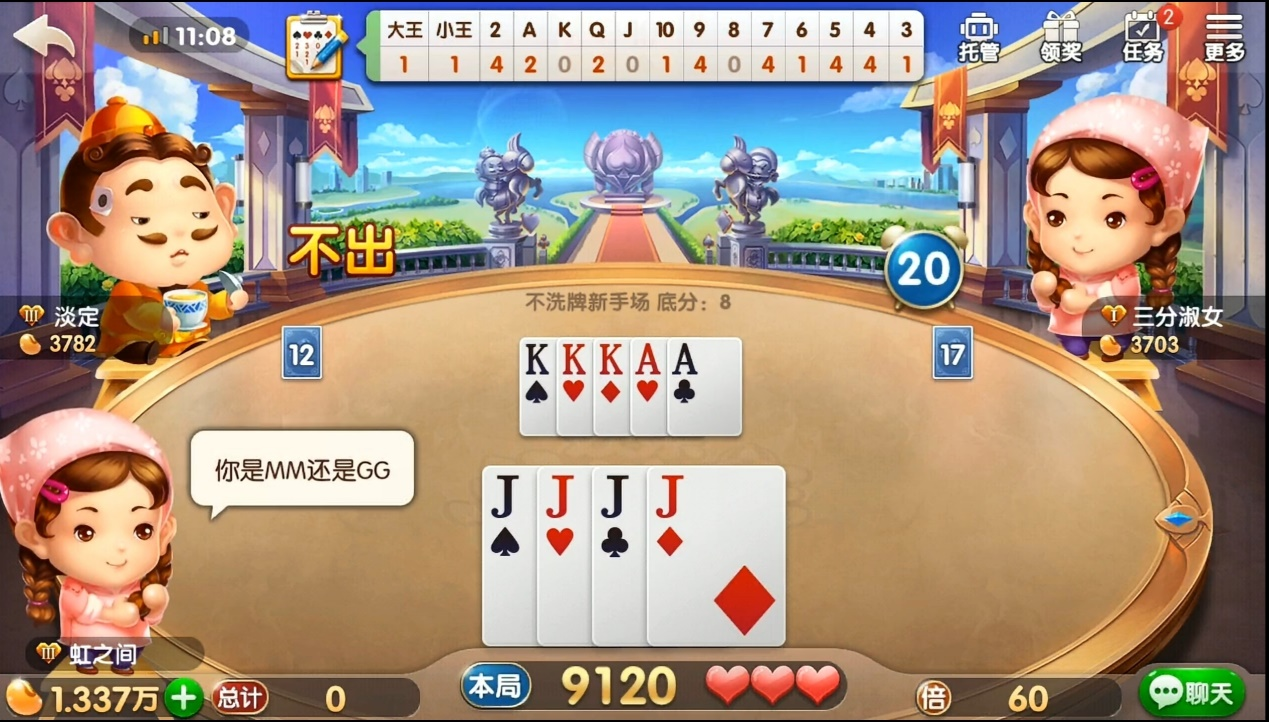
\includegraphics[width=0.75\textwidth]{Figures/game/fight-landlord.jpg}
    \caption{斗地主.}
\end{figure}
\end{example}

我们在本部分主要关注最简单的一种博弈,即\emph{完全信息确定性回合制博弈}\index{博弈!完全信息确定性回合制~}。这样的博弈可以用博弈树表示出来,例如,井字棋的博弈树可以画作\Cref{fig:gametree}.

\begin{figure}
    \centering
    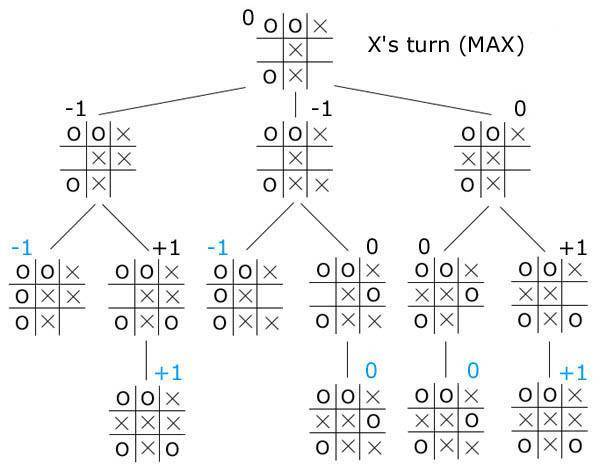
\includegraphics[scale=0.4]{Figures/game/gametree.jpg}\lhysays{重画}
    \caption{井字棋的博弈树}
    \label{fig:gametree}
\end{figure}

\subsection{Zermelo定理与AlphaGo Zero}

输赢博弈一个自然的问题是:玩家是否总可以获胜?这就涉及到\emph{必胜策略}\index{必胜策略}的概念:无论对手如何进行行动,玩家都可以取得胜利的策略. 必胜策略是一种\emph{解概念}\index{解概念},即给定一个博弈,求解具有一定性质的玩家策略. 如果某个玩家具有必胜策略,那么我们就说这个博弈是\emph{被决定的}\index{博弈!被决定的~}. 

什么博弈是被决定的?这一问题的答案由Zermelo定理给出.

\begin{theorem}[Zermelo定理, Von Neumann]\label{thm:zermelo}\index{Zermelo定理}
如果一个博弈是双人的、有限深的、确定的、完全信息的、输赢的,那么这个博弈是被决定的.
\end{theorem}
以上限定词缺一不可,缺少了任何一个都可能导致结论不成立.

\begin{proof}[证明一:逻辑证明]
设$W_i$表示“玩家$i$获胜”, $i=1,2$. 于是$x\in W_1\iff x\not\in W_2$.

先手玩家有必胜策略当且仅当
\[\exists a_0\forall b_0\exists a_1\forall b_1\dots\exists a_n\forall b_n: (a_0b_0\dots a_nb_n)\in W_1.\]

后手玩家有必胜策略当且仅当
\[\forall a_0\exists b_0\forall a_1\exists b_1\dots\forall a_n\exists b_n: (a_0b_0\dots a_nb_n)\in W_2.\]

两个命题互为否定,因此二者恰有一个成立!
\end{proof}

\begin{proof}[证明二:后向归纳法]
从博弈树的叶节点往根节点推理,见图\Cref{???}\lhysays{画个图}.

如果此节点是玩家$i$的回合,那么往后一轮的局面已经完全确定.
\begin{itemize}
    \item 如果有一种走法使得玩家$i$必胜,那么玩家$i$选择这种走法即可.
    \item 否则,玩家$i$无论如何也不可能获胜.
\end{itemize}

当到达到根节点的时候,有一方有必胜策略,另一方必输.

这种证明方式被称为\emph{后向归纳法}\index{后向归纳法}:从最后一期开始往前推理,最终确定策略.
\end{proof}

如果博弈的结局还有平局,我们有如下Zermelo定理:
\begin{theorem}[有平局的Zermelo定理]\label{thm:zermelo-draw}\index{Zermelo定理}
如果一个博弈是双人的、有限深的、确定的、完全信息的,博弈的结果有输赢平局三种,那么下面三条有且仅有一条成立:
\begin{itemize}
    \item 第一个玩家有必胜策略.
    \item 第二个玩家有必胜策略.
    \item 双方都有不败策略.
\end{itemize}
\end{theorem}
证明见习题\lhysays{出一下}。

尽管Zermelo定理的第二个证明构造出了必胜策略,但是后向归纳法的搜索空间过于庞大. 例如,充分大但有限的棋盘上,五子棋先手玩家存在不败策略(见习题\lhysays{出一下}),但是没有经过训练的人类或者简单的算法先手不一定会胜利. 

究其原因,人的思考以及机器搜索的过程实际上是前向探索的过程. 如何进行(启发式)搜索是取得胜利重要的因素. 在本章开头,我们讲述了AlphaGo的故事,这是正是一个很好的例子. 下面我们就如何对围棋进行建模进行讨论.

由Zermelo定理可知,围棋也存在必胜策略. 然而标准围棋棋盘大小为$19\times 19$,状态空间量级为$10^{170}$,过大的状态空间使得我们无法使用后向归纳法求解出必胜策略. 以下我们探讨AlphaGo Zero\index{AlphaGo Zero}(下面简称Zero)如何通过神经网络建模博弈的过程.

首先,我们假定Zero可以记住的是从当前局开始往前$k$步的棋局信息(即落子方式)。我们假定这样的$k$步棋形成的棋局序列集合为$C$. 于是,Zero的策略是一个随机映射
\[\pi: C\to \Delta(\mathcal A),\]
其中$\mathcal A$是所有可能的落子方式的集合,而$\Delta(\mathcal A)$是$\mathcal A$上的概率分布. 这里,我们假定Zero的策略是一个随机策略,而非确定性策略。此时,概率分布$\pi(s)$表示在状态$s$下,Zero选择对应的落子方式的似然\index{似然}(或者对胜利的自信程度).

最后,当博弈结束时,Zero会获得一定的收益,我们假定Zero赢的时候收益为$+1$,输的时候收益为$-1$. 

对于人类来说,我们的任务是让Zero的策略$\pi$尽可能地接近必胜策略,为此,我们需要用一个神经网络来拟合这个策略. 此外,我们通常需要告诉Zero每一步棋获胜的概率(或者说期望收益),这也需要一个神经网络。具体来说,AlphaGo Zero算法包含\emph{策略网络}\index{策略网络},\emph{价值网络}\index{价值网络}和\emph{Monte-Carlo树搜索}(MCTS)\index{Monte-Carlo树搜索}\index{MCTS}.
\begin{itemize}
    \item 策略网络$p$和价值网络$v$的输入为当前状态$s\in C$,即$(P(s,\cdot),V(s))=f_\theta(s)$.
    \item 策略网络$P(s,\cdot)$的输出为下一步落子位置$a\in\mathcal A$的概率分布.
    \item 价值网络$V(s)$的输出为该状态的价值评估(期望收益、胜率).
    \item MCTS利用策略网络进行\emph{扩展},使用价值网络进行\emph{评估},利用UCB公式返回最优的搜索结果作为落子决策.
\end{itemize}

Zero使用强化学习(自博弈,策略梯度)的方式训练策略网络,使用自我博弈过程中的数据监督训练价值网络. 这个过程如\Cref{fig:alphago-zero} 所示.

\begin{figure}[ht]
\centering
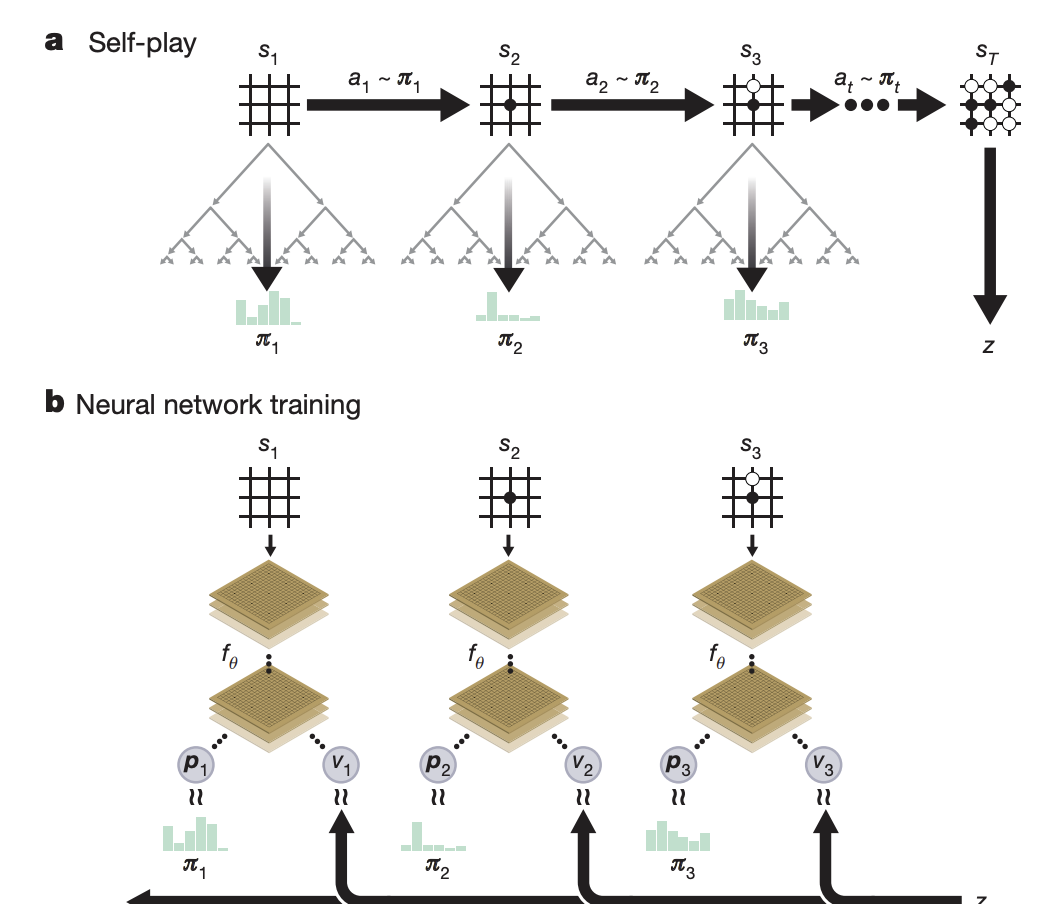
\includegraphics[width=0.7\textwidth]{Figures/game/alphazero.png}\lhysays{重画}
    \caption{AlphaGo Zero的训练过程}
    \label{fig:alphago-zero}
\end{figure}

在开始细节之前,我们先给一个比喻,看看整个流程是如何模拟人类学习的. 假设Zero是一个人。
\begin{itemize}
    \item 他可以按照他的技术水平(即启发式搜索函数)在脑中模拟一场围棋比赛,并且假定对手和自己一样聪明。最终,这一模拟会有一个结果(输或者赢),这一结果反映了他的策略的好坏. 这就是用MTCS自博弈的过程.
    \item 假设他在脑中模拟了很多场比赛,他可以把这些比赛记录下来,然后根据这些记录来调整自己的策略,并调整自己对于胜率的评判. 这就是策略网络和价值网络的训练过程.
    \item 他可以不断重复上面两个过程,来精进自己的技术水平。
\end{itemize}

下面,我们逐步解释Zero的训练过程.

\begin{itemize}
    \item 自博弈过程$s_1,\cdots,s_T$: 在每个状态$s_t$, 使用最近一次的网络$f_\theta$,执行一次MCTS $\alpha_\theta$(具体过程见后面). 下法根据MCTS计算的搜索概率$\pi_t$来选择,$a_t\sim\pi_t$. 最后,依据围棋规则,对终止状态$s_T$打分,来计算胜利者$z$. 
    \item 神经网络训练: 使用原始的棋盘状态$s_t$作为输入,输出$(p_t,v_t)=f_\theta(s)$,表示当前玩家在$s_t$的策略和胜率. 训练时更新网络参数$\theta$,以最大化策略$p_t$和搜索概率$\pi_t$的相似性,并最小化预测赢家$v_t$与实际赢家$z$的误差. 新参数将应用于下一次自博弈$a$的迭代.     
\end{itemize}

MTCS的过程较为复杂,我们单独介绍。树的组成如下:搜索节点是状态$s$,边是状态-行动对$(s,a)$. 每条边需要存储以下信息:
\begin{itemize}
    \item $N(s,a)$:边的访问次数.
    \item $P(s,a)$:策略网络在状态$s$中选择行动$a$的概率.
    \item $Q(s,a)$:动作价值,$Q(s,a)=\frac{1}{N(s,a)}\sum_{s':s,a\to s'} V(s')$,其中$V$是价值网络. 这一值反映了在状态$s$选择行动$a$的平均收益.
\end{itemize}

接下来,MTCS要做如下迭代(见\Cref{fig:mcts}):
\begin{itemize}
  \item 从根节点开始,状态$s$固定,选择具有最大的 $Q(s,a) + U(s,a)$的分支。
  \begin{itemize}
    \item $U$ 是上限置信度,$U(s,a)\propto{P(s,a)}/(1+N(s,a))$.
    \item $Q+U$是置信区间的上界,称为UCB公式。
  \end{itemize}
  这一过程其实就是在模拟自己和对手的多轮行动,其中选择$Q+U$最大的分支即是启发式搜索的形式。

  \item 当选到叶节点时,扩展叶节点。使用神经网络 $f_\theta(s)$ 来计算新的$P(s,a)$和$V(s)$,并把$P$存储到对应的边上. 只要还可以扩展,就说明还有一方玩家可以继续行动,所以这一过程可以持续到有一方获胜或者到达最大深度.

  \item 根据 $V$ 更新动作价值 $Q$,反映所有该动作的子树的平均值. 这反应了此次模拟的结果如何影响这一动作的评价:输了的话,这一动作的评价会降低,赢了的话,这一动作的评价会提高.

  \item 一旦搜索结束,返回搜索概率 $\pi$,$\pi(a)$正比于$N(s,a)^{1/\tau}$,$\tau$ 是一个参数,控制着温度. 温度反映了$\pi$允许的随机性程度,当$\tau$趋于正无穷的时候,$\pi$趋于均匀分布,当$\tau$趋于零的时候,$\pi$趋于一个退化分布,以概率$1$取最大$N(s,a)$对应的$a$.
\end{itemize}

\begin{figure}[ht]
\centering
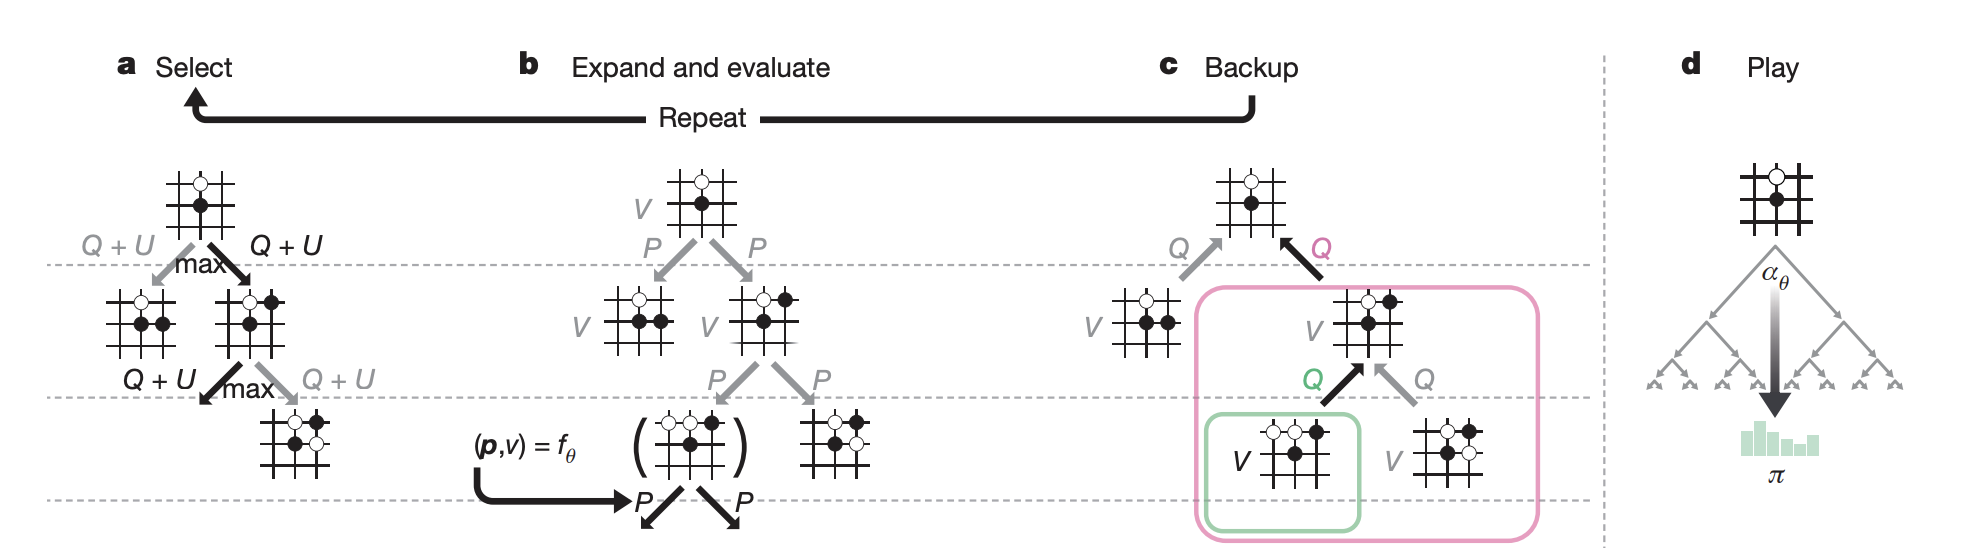
\includegraphics[width=0.7\textwidth]{Figures/game/mcts.png}\lhysays{重画}
    \caption{MCTS的过程}
    \label{fig:mcts}
\end{figure}

\section{正则形式博弈}
输赢博弈被建模为\emph{扩展形式博弈}\index{博弈!扩展形式~},它代表了多轮博弈的过程. 与之相对的是\emph{正则形式博弈}\index{博弈!正则形式~},即玩家只有一次行动的机会,所有玩家同时操作. 正则形式博弈通常要求信息是完全的. 那么,如何定义正则形式博弈和对应的解概念呢?

\subsection{定义}

我们直接给出一个很直观的的模型。

\begin{definition}[正则形式博弈]\index{博弈!正则形式~}
一个\textbf{正则形式博弈}由以下要素构成:
\begin{itemize}
    \item 玩家集合:$I$,我们总是假设这是一个有限集合.
    \item 玩家的行动空间:$A_i$,$i\in I$.
    \item 玩家的收益:$u_i:\prod_j A_j\to\R$.
\end{itemize}
\end{definition}

有以下特殊的正则形式博弈:
\begin{itemize}
    \item 当$A_i$有限,我们称之为\emph{矩阵博弈}\index{博弈!矩阵~}. 之所以称为矩阵博弈,是因为我们可以用一个矩阵来表示玩家的收益. 
    
    比如,考虑$|I|=2$,即有两个玩家,$|A_1|=m,|A_2|=n$,那么要确定$u_i$只需要确定$u_i(a_1,a_2)$的值,这恰好就是一个$m\times n$的矩阵. 此时,我们将第一个玩家称之为\emph{行玩家},第二个玩家称之为\emph{列玩家}.

    对于更多玩家的博弈,尽管$u_i$不再可以被矩阵表示,但上面的这一表示的思路依然适用,所得到的结果在线性代数上称之为\emph{张量}\index{张量}. 但是遵循传统习惯,我们依然把这种博弈称之为矩阵博弈.

    \item 当$A_i$是$\R^n$的连通子集且和$u_i$都是连续的,我们称之为\emph{连续博弈}\index{博弈!连续~}.
    \item 当$\sum_i u_i=0$,我们称之为\emph{零和博弈}\index{博弈!零和~}. 一般地,如果存在常数$c$使得$\sum_i u_i=c$,我们称之为\emph{常和博弈}\index{博弈!常和~}. 常和博弈和零和博弈通常具有一致的性质,所以我们也把常和博弈视为零和博弈. 如果$u_i$只有两个取值(例如$-1,1$),我们称之为\emph{输赢博弈}\index{博弈!输赢~}.
\end{itemize}

下面,我们看两个典型的例子。

\begin{example}[囚徒困境]\index{囚徒困境}\label{ex:prisoner}
在囚徒困境中,一共有两个玩家,行玩家和列玩家. 玩家的第一个选择是保持沉默,第二个选择是认罪并检举对方. 它有如下收益矩阵:
\[
\begin{pmatrix}
-1,-1&-10,0\\
0,-10&-5,-5\\
\end{pmatrix}.
\]
矩阵每一项第一个元素是行玩家的收益,第二个是列玩家的收益. 显然,这是一个非零和的矩阵博弈。

在这个例子中,博弈的属性非常鲜明:每个人的收益不仅仅取决于自己的选择,还取决于对方的选择. 因此,玩家在做决策时,必须要考虑对方玩家可能会如何行动。
\end{example}

\begin{example}[猜硬币游戏]\index{猜硬币游戏}
在猜硬币游戏中,行列玩家分别有一枚硬币,他们秘密地抛掷. 如果两个玩家的硬币上面相同,行玩家获胜;否则列玩家获胜. 收益矩阵为:
    \[
    \begin{pmatrix}
    1,0&0,1\\
    0,1&1,0\\
    \end{pmatrix}.
    \]
容易验证,这个博弈是一个零和博弈,进一步,是一个输赢博弈.
\end{example}

至于连续博弈的例子,这里我们先略过。我们会在后面详细讨论\emph{生成对抗网络}\index{生成对抗网络},它是一个连续博弈的例子.

现在,我们有了博弈,接下来的任务就是定义\emph{策略}\index{策略}. 假设所有人之间是不能交流的,每个人独立做决策,因此玩家之间不能协调彼此的决策. 所以,我们可以很简单地定义玩家$i$的策略$s_i$为行动空间$A_i$的一个元素。将所有玩家的策略收集起来,我们就得到了\emph{策略组合}\index{策略组合}:
\[
s=(s_i)_{i\in I}.
\]

\subsection{理性与均衡}

接下来,我们要定义正则形式博弈中的解概念,换言之,玩家最终会如何进行这场博弈并获得对应的收益。这里,我们将引入博弈论中两个重要的概念:\emph{理性}\index{理性}和\emph{均衡}\index{均衡}。

尽管理性这一词已经被广泛使用,但是,究竟什么是理性依然是一个有巨大争议的问题. 比如,我们考虑这些定义,以及让他们变得很微妙的场景:
\begin{itemize}
    \item 理性指的是无穷的信息获取能力。我们把理性玩家处在一个到处都是抛硬币的世界,他怎么做才算理性?
    \item 理性是无穷的计算资源。我们知道,这个世界上存在一些数学命题(记为$p$)虽然有真假,但是我们既不能证明它,也不能证伪它(Gödel第二不完备性定理\index{Gödel第二不完备性定理}). 现在,我们给理性玩家设计一个博弈,如果证明了$p$,他就赢,否则他就输. 这个玩家怎么做才算理性?
\end{itemize}

以上两种对于理性的理解只是冰山一角。这里通过这些例子想说明,理性是一个非常复杂的概念,我们很难达成一个共识。因此,更加务实的做法是,我们不去讨论理性的定义,而是直接给出一个理性的定义,然后看看这个定义下会发生什么.

\emph{均衡}这一概念正是诞生于这样的背景下. 所谓均衡,指的是在某种理性的前提下,面对其他玩家,每个人都做出了他能做出的最优选择,这种最优选择被称为\emph{最优反应}\index{最优反应}. 因此,所有人互相都是最优反应的时候,就构成了一个均衡.

上面的讨论总结起来就是如下的对应关系:

\[
\text{理性}\iff\text{最优反应}\iff\text{均衡}.
\]
博弈论的核心就在于研究以上三个概念之间的关系.

以上讨论比较抽象和一般,我们现在回到正则形式博弈,看看在这个背景下,这三个概念是如何定义的.

首先,理性的定义是非常简单的:在玩家知道其他玩家的信息(即策略)之后,他会最大化自己的收益。然后,在这一定义下,最优反应可以自然定义如下:

\begin{definition}[最优反应]\index{最优反应}
给定对手的策略组合$s_{-i}$,玩家$i$的\textbf{最优反应}是一个策略$s_i$,满足对任意$a_i\in A_i$,
    \[u_i(s_i,s_{-i})\geq u_i(a_i,s_{-i}),\]
即玩家$i$的收益最大化. 最优反应对应的策略集合记为$BR_i(s_{-i})$.
\end{definition}
这里,$s_{-i}$表示除了玩家$i$之外的所有玩家的策略组合,我们将会频繁使用这个记号.

最后,我们定义均衡的概念,我们很自然有如下的定义:

\begin{definition}[纯策略Nash均衡]\index{Nash均衡!纯策略~}
\textbf{纯策略Nash均衡}指的是策略组合$s$,对任意玩家$i$和任意$a_i\in A_i$,有
    \[u_i(s_i,s_{-i})\geq u_i(a_i,s_{-i}).\]
\end{definition}

我们也可以用不动点(见\Cref{chap:fixed-point-theory})来理解纯策略Nash均衡. 纯策略Nash均衡的等价定义是每个人都达到了自己的最优反应,即最优反应的不动点. 更一般地,任何一个均衡的概念都可以理解为最优反应对应的不动点.

作为一个例子,我们继续考虑囚徒困境.
\begin{example}[囚徒困境的纯策略Nash均衡]\index{囚徒困境}
回忆\Cref{ex:prisoner},它有如下收益矩阵:
\[
\begin{pmatrix}
-1,-1&-10,0\\
0,-10&-5,-5\\
\end{pmatrix}.
\]
矩阵每一项第一个元素是行玩家的收益,第二个是列玩家的收益. 

这个博弈有唯一的纯策略Nash均衡:每个人都认罪(第二行),此时大家都会获得$-5$的收益. 比如,行玩家选择第一行,那么,无论列玩家选了第一列还是第二列,行玩家都会选择第二行,因为这样他的收益更高. 同理,列玩家也是如此. 因此,这个策略组合是一个唯一的纯策略Nash均衡.

注意,如果两个选择都是保持沉默,那么他们的收益会更高($-1$),但他们却无法达到这个收益。这正是我们定义的理性所蕴含的意义:在博弈中,每个人都是自私的,如果知道了对方的选择,他们会选择最优的策略,而不会稍微放弃一点自己的利益,以换取博弈双方更大的利益.
\end{example}

然而,我们继续猜硬币游戏\index{猜硬币游戏},我们会发现这个博弈没有纯策略Nash均衡. 回忆,这一博弈的收益矩阵为:
    \[
    \begin{pmatrix}
    1,0&0,1\\
    0,1&1,0\\
    \end{pmatrix}.
    \]
我们现在验证,这个博弈没有纯策略Nash均衡. 如果行玩家选择第一行,那么列玩家的最优反应是第二列,然而,此时行玩家的最优反应是第二行;而行玩家选择第二行的情况类似。因此,无论如何选,最优反应都不可能形成一个不动点(即均衡).

更一般地,二人正则形式输赢博弈中纯策略Nash均衡往往不存在. 我们有如下定理:
\begin{theorem}
设$G=(I,\{A_i\}_{i\in I}, \{u_i\}_{i\in I})$是一个二人正则形式输赢博弈,其中$I=\{1,2\}$. 那么,$G$存在纯策略Nash均衡当且仅当其中一个玩家存在必胜策略. % HW:证明这个定理的矩阵博弈形式
\end{theorem}
证明见习题\lhysays{出一下}.

对比动态博弈中的Zermelo定理,静态的二人完全信息输赢博弈已经不能够保证必胜策略的存在性. 因此,静态输赢博弈的结局往往比动态输赢博弈更加不确定.


\subsection{生成对抗网络}

接下来,我们给一个连续博弈的例子,即\emph{生成对抗网络}\index{生成对抗网络}(GAN)\index{GAN}. 生成对抗网络由两个子模型组成,一个被称为\emph{\index{生成模型}生成模型},一个被称为\emph{\index{判别模型}判别模型}. 生成模型的任务是生成看似真实的数据,而判别模型的任务是识别给定的数据是真实的还是伪造的. 这一过程的示意见图\Cref{???}\lhysays{画一下}.

假设真实数据的分布为$F_{data}$. 
\begin{itemize}
    \item 生成模型为$G(x;\theta_g)$,参数为$\theta_g$,输入随机向量$x$,输出数据向量$z$。当$x$服从分布$F_x$,$G$的输出会形成一个分布$F_g$。
    \item 判别模型为$D(z;\theta_d)$,参数为$\theta_d$,接受一个数据向量$z$,输出一个$[0,1]$中的实数,表示$z$来自分布$F_{data}$的概率(似然\index{似然}).
\end{itemize}
我们假设$F_{data}$和$F_x$都是连续型分布,有密度函数$p_{data}$和$p_x$. 我们再假设$D$和$G$都是连续的.

将$G$和$D$看成两个玩家,于是GAN可以被看成一个二人零和博弈,收益函数为:
    \[
        V(G,D)=\E_{z\sim F_{data}}(\log D(z))+\E_{x\sim F_x}(\log(1-D(G(x)))).
    \]
$D$最大化$V$,$G$最小化$V$.

接下来,我们要解释,为什么这个收益函数能够达到我们的目标. 我们有以下三点讨论:

\begin{itemize}
    \item 一方面,如果$D$越厉害,那么$D$会尽可能地把真实数据和生成数据区分开,$1-D(G(x))$也会更大,因此$V$会更大. 另一方面,如果$G$越厉害,那么$D$会更容易把真实数据和生成数据混淆,于是$1-D(G(x))$会更小,$V$也会更小. 因此,$D$和$G$之间是一个对抗的关系.
    
    \item 如果收益函数只有第二项,判别器$D$可以“作弊”,即无论输入什么都判定为假,这样他总是能得到最大的收益. 为了避免这种情况,我们引入了第一项,即真实数据的似然. 这样,$D$还需要努力判断真实数据,而不是只判断生成数据.
    
    \item 为什么$V$是对数的形式?在\Cref{chap:information-theory} 中我们解释过,这样形式的收益函数是交叉上损失函数的形式. 因此这一损失函数可以衡量两个分布之间的相似性,对于随机的数据来说,这是一个比较好的衡量方式.
\end{itemize}


从博弈论角度出发,一个基本的问题是Nash均衡是否存在?假设$D$和$G$都可以任意选择连续函数. 我们将展示一种通用的方式求解连续博弈的Nash均衡. 注意到$G(x)$形成了一个连续分布,密度记为$p_g$.  首先证明密度函数存在性定理:
\begin{theorem}
设$X\sim \mathcal U(0,1)$. 对于任意密度函数$p$,存在一个连续函数$F$使得$F(X)$具有密度$p$.
\end{theorem}
\begin{proof}
设$F_p$是$p$对应的分布函数,它是一个单调的连续函数. 取$F(x)=\inf\{y\in \R: F_p(y)\geq x\}$即可.
\end{proof}
因此,$G$的行动等价于选择$p_g$.

给定$G$的选择$p_g$,我们来求$D$的最优反应$D^*$.
    \[V(G,D)=\int (p_{data}(x)\log D(x)+p_g(x)\log(1-D(x)))\d x.\]
函数$a\log x+b\log(1-x)$最大值在$x=a/(a+b)$的时候取得. 因此,
    \[D^*(x)=\frac{p_{data}(x)}{p_{data}(x)+p_g(x)}.\]
    
现在,给定最优反应$D^*=p_{data}(x)/(p_{data}(x)+p_g(x))$,我们来求$G$的最优反应. 直观上,$G$能做到的最好选择就是$p_g=p_{data}$. 此时,$D^*(x)=1/2$,因此对任意$G$,$V(G,D^*)=-\log 4$. $G$选任何策略都是一样的收益,因此这是一个Nash均衡. 我们证明了:
\begin{theorem}[GAN的Nash均衡存在性]
在GAN的博弈中,$G$选择$p_{data}$,$D$选择$1/2$是一个Nash均衡.
\end{theorem}
这一证明见习题\lhysays{出一下}.

\subsection{混合策略}
我们已经看到,在相当普遍的情况下,纯策略Nash均衡并不存在. 所以我们需要允许玩家进行随机行动,这就是\textbf{混合策略}\index{混合策略}. 

\begin{definition}[混合策略]\index{混合策略}
给定一个正则形式博弈$G=(I,\{A_i\}_{i\in I},\{u_i\}_{i\in I})$,其中$I$是玩家集合,$A_i$是玩家$i$的行动空间,$u_i$是玩家$i$的收益函数. 玩家$i$的行动空间上的概率分布集合为$\Delta(A_i)$. 那么,玩家$i$的\textbf{混合策略}是一个概率分布$\sigma_i\in\Delta(A_i)$。
\end{definition}

当$A_i$有$n$个元素(有限),$\Delta(A_i)$可以被表示为标准的$n$-单纯形\index{单纯形}:
    \[\Delta(A_i)=\left\{x\in\R^n:\sum_{i=1}^n x_i=1,\forall j,x_j\geq 0\right\}.\]

特别地,纯策略可以被看成是一个特殊的混合策略,即退化的概率分布.

有了混合策略,我们还需要重新定义玩家的理性。一个非常标准的回答是\emph{期望效用理论}\index{期望效用理论},它由Von Neumann和Morgenstern提出. 该理论认为,在面对不确定性时,人按照期望效用进行决策. 


因此,我们需要计算玩家的期望效用. 为此,引入混合\emph{策略组合}\index{策略组合}:$\sigma=(\sigma_i)_{i\in I}$,其中$\sigma_i\in\Delta(A_i)$. $\sigma$是一个$(A_i)_{i\in I}$上的概率分布,每一维相互独立. 当所有玩家选定策略之后,玩家$i$的期望收益是:
    \[u_i(\sigma)=\E_{a\sim\sigma} u_i(a).\]

有了期望效用,我们可以重新定义最优反应:

\begin{definition}[最优反应]\index{最优反应}
给定对手的策略组合$\sigma_{-i}$,玩家$i$的\textbf{最优反应}是一个策略$\sigma_i$,满足对任意$\sigma_i'\in \Delta(A_i)$,
    \[u_i(\sigma_i,\sigma_{-i})\geq u_i(\sigma_i',\sigma_{-i}),\]
即玩家$i$的期望收益最大化. 最优反应对应的策略集合记为$BR_i(\sigma_{-i})$.
\end{definition}

最后,我们可以重新定义均衡的概念:

\begin{definition}[Nash均衡]\index{Nash均衡}
对于一个博弈$G=(I,\{A_i\}_{i\in I},\{u_i\}_{i\in I})$,如果混合策略组合$\sigma$满足对于任意玩家$i$和任意$\sigma_i'\in \Delta(A_i)$,都有
\[u_i(\sigma_i,\sigma_{-i})\geq u_i(\sigma_i',\sigma_{-i}),\]
那么,$\sigma$是一个\textbf{Nash均衡}.
\end{definition}

同样,Nash均衡也可以理解为最优反应的不动点. 利用这一观点,Nash得以使用不动点定理证明了Nash均衡的存在性:
\begin{theorem}[Nash均衡存在性定理]\index{Nash均衡存在性定理}
任意有限正则形式博弈都存在一个Nash均衡.
\end{theorem}

\begin{remark}
    目前为止,我们一共定义了两种均衡:纯策略Nash均衡和Nash均衡。后一种均衡实际上应该被称作\emph{混合策略Nash均衡}\index{Nash均衡!混合策略~},但是为了和文献统一,我们直接称之为Nash均衡,而忽略前缀“混合策略”.

    实际上,按照我们理性-最优反应-均衡的思路,Nash均衡和纯策略Nash均衡是本质不同的两种均衡:前者引入了期望效用理论来体现玩家面对不确定性时候的行为,而后者则是直接最大化,没有不确定性。因此,我们并不能简单说前者是后者的推广。
\end{remark}

我们来看一个例子. 
\begin{example}[猜硬币游戏的Nash均衡]
继续考虑猜硬币游戏\index{猜硬币游戏},收益矩阵为
\[
\begin{pmatrix}
1,0&0,1\\
0,1&1,0\\
\end{pmatrix}.
\]

我们接下来证明,唯一的Nash均衡是两个玩家都选择$(1/2,1/2)^\t$,即两个玩家都以等概率来猜硬币的正反面. 我们有如下分类讨论:
\begin{itemize}
    \item 两个玩家都是纯策略:我们之前已经说明,这个博弈没有纯策略Nash均衡. 
    \item 行玩家是纯策略而列玩家的策略是$(p,1-p)^\t$,其中$p\in(0,1)$. 考虑行玩家的期望收益:
    \[
        u_1(\sigma_1,\sigma_2)=\begin{cases}
            p,&\text{$\sigma_1$是第一行},\\
            1-p,&\text{$\sigma_1$是第二行}.
        \end{cases}
    \]
    因此,如果$p>1/2$,行玩家会选择第一行,但此时列玩家的最优反应是选择第二列,因此这不是一个Nash均衡. 同理,如果$p\leq 1/2$,也不是一个Nash均衡. 因此,这种情况也不是一个Nash均衡.
    \item 列玩家是纯策略而行玩家的策略是$(p,1-p)^\t$,其中$p\in(0,1)$. 同理,这种情况也不是一个Nash均衡.
    \item 行玩家的策略是$\sigma_1^*=(p,1-p)^\t$,列玩家的策略是$\sigma_2^*=(q,1-q)^\t$,其中$p,q\in(0,1)$. 这种情况下,要确定$p,q$的值计算会很复杂。所以我们这里介绍一个技巧。
    
    注意到,行玩家的任意一个混合策略可以写作
    \[\sigma_1=p_1a_1+p_2a_2,\]
    其中$p_1+p_2=1$,$a_1$和$a_2$是两个纯策略. 因此,在Nash均衡下,对任意$p_1,p_2$,
    \[
    \begin{aligned}
        u_1(\sigma_1^*,\sigma_2^*)&=pu_1(a_1,\sigma_2^*)+(1-p)u_1(a_2,\sigma_2^*)\\
        &\geq p_1u_1(a_1,\sigma_2^*)+p_2u_1(a_2,\sigma_2^*).
    \end{aligned}
    \]
    取$p_1=1$,$p_2=0$,我们有
    \[pu_1(a_1,\sigma_2^*)+(1-p)u_1(a_2,\sigma_2^*)\geq u_1(a_1,\sigma_2^*).\]
    同理,取$p_1=0$,$p_2=1$,我们有
    \[pu_1(a_1,\sigma_2^*)+(1-p)u_1(a_2,\sigma_2^*)\geq u_1(a_2,\sigma_2^*).\]
    注意到,两个不等式的左边其实是右边的加权平均,平均值不小于任何一方,因此这两个不等式实际上是等号. 因此,我们有
    \begin{align*}
        &u_1(a_1,\sigma_2^*)=u_1(a_2,\sigma_2^*)\\
        \iff& q\cdot 1+(1-q)\cdot 0=q\cdot 0+(1-q)\cdot 1\\
        \iff& q=\frac{1}{2}.
    \end{align*}
    同理,我们有$p=1/2$. 因此,双方都选择$(1/2,1/2)^\t$是唯一的Nash均衡.
\end{itemize}
如此,我们证明了猜硬币游戏的唯一Nash均衡是双方都选择$(1/2,1/2)^\t$.
\end{example}

在上面的例子中,我们实际上得到了一个非常重要的结论:Nash均衡具有\emph{无差别原理},它说明,Nash均衡中出现的那些行动一定都是取到了最大收益的行动. 这一原理可以被用来求解任意二人博弈的Nash均衡(见习题\lhysays{出一下}).

\begin{theorem}[无差别原理]\index{无差别原理}
考虑一个正则形式博弈$G=(I,\{A_i\}_{i\in I},\{u_i\}_{i\in I})$,其中$I$是玩家集合,$A_i$是玩家$i$的行动空间,$u_i$是玩家$i$的收益函数. 如果$\sigma^*$是一个Nash均衡,那么对于任意玩家$i$和任意$a_i,a_i'$满足
\[\sigma^*_i(a_i)>0,\quad \sigma^*_i(a_i')>0,\]
有
\[u_i(a_i,\sigma^*_{-i})=u_i(a_i',\sigma^*_{-i})=u_i(\sigma^*)=\max_{\sigma_i\in\Delta(A_i)}u_i(\sigma_i,\sigma^*_{-i}).\]
\end{theorem}

上面我们说明,\emph{有限}正则形式博弈一定有Nash均衡,实际上,类似的不动点技术可以被用来证明更一般的均衡存在定理:

\begin{theorem}[Debreu-Glicksberg-Fan定理]
    一个正则形式博弈满足如下所有条件,就会存在一个纯策略Nash均衡: 
    \begin{itemize}
        \item 对任意玩家$i$,行动空间$A_i$是Euclid空间中的非空紧凸子集,
        \item 对任意玩家$i$,收益函数$u_i$连续,对第$i$个分量上凹。
    \end{itemize}
\end{theorem}

\begin{theorem}[Glicksberg定理]
    一个正则形式博弈满足如下所有条件,就会存在一个Nash均衡:
    \begin{itemize}
        \item 对任意玩家$i$,行动空间$A_i$是度量空间中的非空紧子集,
        \item 对任意玩家$i$,收益函数$u_i$连续。
    \end{itemize}
\end{theorem}

尽管在数学上,期望效用理论导出了漂亮的结果,即Nash均衡的存在性,但是(期望)效用理论非常不符合实验的观察. 比如说,下面两个选项,大部分人会更倾向于选择第一个:
\begin{itemize}
    \item 你得到1000元.
    \item 你有1\%的概率得到100000元,99\%的概率得到0元.
\end{itemize}
然而,如果我们套用期望效用理论,两个选项的期望效用是一样的!

此外,从某种角度来看,价值也是相对的。如果我们有 50\% 的机会赢 100 块钱或 10 块钱,拿到 10 块钱时可能会感到失望。但如果改成我们只能赢得 10 块钱或 1 块钱,那得到 10 块钱时我们就会感到更开心. 因此,即便效用理论是对的,在现实中我们完全不能知道真正的效用函数是什么,也无法在现实中真的用来建模.

那么,为什么我们还要研究(期望)效用理论,甚至整个经济学和博弈论的体系都是基于(期望)效用理论的?它之所以如此重要,就是因为它很好地平衡了“可以写理论结果”和“可以解释现实现象”之间的关系. 正如Robert Aumann所说,

\begin{quotation}
    “另一种强调这一点的原因——即理论不应简单地被视为真或假——是为了避免过分抠字眼带来的问题……有人反对效用最大化的概念,认为人并不真的在最大化效用。对此,有人提出了诸如‘满意准则’这样的替代方案……然而,\emph{效用最大化的有效性并不在于它能否精确描述个体行为,而在于它作为经济理论的基础假设,能够整合大量经济学理论}……

    “像‘满意准则’这样的替代方案虽然看起来有吸引力,但几乎没有什么实际作用,它们很少带来有趣的结果。在评价效用最大化时,我们不应问‘它是否合理?’,而是应该问‘它能整合什么?它能引导我们走向哪里?’”
\end{quotation}

在任何时候,作为一门语言,博弈论都应该具备Aumann所说的这种特性. 我们不能为了数学的方便而过分简化理论,但更不能过分拟合现实,变得毫无指导和应用价值.

\section{随机博弈(Markov博弈)}
现在我们考虑无穷博弈中最简单的一种:\textbf{随机博弈}\index{博弈!随机~},也叫\textbf{Markov博弈}\index{博弈!Markov~}. 在随机博弈中,玩家的行动是随机的,但是玩家的行动空间是有限的. 为了简化问题,我们考虑两人随机博弈,即两个玩家轮流进行随机行动. 其相关概念如下:
\begin{itemize}
    \item 有限局面:$C=\{s_1,s_2,\cdots,s_N\}$.
    \item 有限策略:$\mathcal A=\mathcal A_1\times \mathcal A_2.$
    \begin{itemize}
        \item 每个局面具有自己的行动空间:$\mathcal A_p = \{\mathcal A_{p,1},\mathcal A_{p,2},\cdots, \mathcal A_{p,N}\}, (p=1,2)$.
        \item 每个行动空间有限:$|\mathcal A_{p,k}|=n_{p,k},(p=1,2;k=1,2,\cdots,N)$.
    \end{itemize}
    \item 在局面$s_k$, 若玩家1选择第$i$个行动$a_{1,k,i}(1\leq i\leq n_{1,k})$,玩家2选择第$j$个行动$a_{2,k,j}(1\leq j\leq n_{2,k})$,则
    
    \begin{itemize}
        \item 局面之间有转移概率:
        \begin{itemize}
            \item 该博弈以概率$s_{ij}^k$停止.
            \item 该博弈以概率$p_{ij}^{kl}$转移到状态$s_l$.
        \end{itemize}
        \item 收益:玩家1收获$Q(a_{1,k,i},a_{2,k,j};s_k)$,玩家2收获$-Q(a_{1,k,i},a_{2,k,j};s_k)$. 假设$Q$有界.
    \end{itemize}
\end{itemize}

随机博弈的过程如下. 首先,博弈从某一个局面状态$s^0$开始,$s^0\in C$. 在每个阶段$t$,所有玩家同时选择自己的动作$a^t$. 环境根据所有玩家的动作$\boldsymbol a^t$和状态$s^t$,给予每个玩家对应的收益$q(\boldsymbol a^t, s^t)$,并转移到新的状态$s^{t+1}\in C$. 

假设在阶段$T$,所有玩家可以观察到所有历史动作$\{\boldsymbol a^t\}_{t\leq T}$. 和一般的动态博弈一样,我们可以定义每个玩家的策略$\pi$——基于历史信息(状态、行动)到当前局面的行动的映射. 玩家在博弈的过程中,其实就是按照某个策略$\pi$进行行动的. 求解一个博弈也是求解最优策略$\pi_*$. 下面我们定义什么是``最优".

依赖历史信息的策略$\pi$一般很复杂. 由于收益只与当前局面、当前玩家的行动有关,我们可以缩小策略空间. 考虑第$p$个玩家($p=1,2$),定义\emph{平稳策略}\index{平稳策略}为$N$个概率分布:$\vec \pi_p=(\pi_p^1,\pi_p^2,\cdots,\pi_p^N)$,分别对应$N$个状态;每个概率分布$\pi_p^k=(\pi_{p,1}^k,\pi_{p,2}^k,\cdots,\pi_{p,n_{p,k}}^k)$,分别对应$|n_{p,k}|$个行动. 使用平稳策略时,无论博弈的历史轨迹如何,玩家$p$在状态$s_k$采取行动$a_{p,k,i}$的概率为$\pi_{p,i}^k$.

假设两个玩家分别用平稳策略$\pi_1,\pi_2$进行博弈,则从局面$s^0$开始的随机博弈中,第$p$个玩家($p=1,2$)的\emph{远期收益}\index{远期收益}:
        \[\Pi_p(\pi_1,\pi_2; s^0) = \E\left[\sum_{t=0}^\infty \gamma^t(-1)^{p-1} Q(\pi_1(s^t),\pi_2(s^t); {s^t}) \right].\]

以上定义容易扩展为一般随机博弈(多人、非零和). 随机博弈可以看做MDP的多人扩展$(N, C, \mathcal A, \mathcal P,\mathcal Q, \gamma)$:
\begin{itemize}
    \item $N$: 玩家的数量,$N=1$退化为MDP.
    \item $C$: 局面的集合.
    \item $\mathcal A$: 玩家的行动空间合. $\mathcal A=\mathcal A^1\times \cdots\mathcal A^N$. 设$\mathcal A_i(s)$表示第$i$个玩家在状态$s$的行动空间.
    \item $\mathcal P: C\times \mathcal A\times C\to [0,1]$: 给定玩家的联合动作$\boldsymbol a\in\mathcal A$, 局面从状态$s\in C$转移到$s'\in C$的概率$P(s'|s,\boldsymbol a)$.
    \item $\mathcal Q: C\times \mathcal A\to \R$: 在状态$s$,当玩家的联合动作为$\boldsymbol a$时,玩家$i$的奖励值$Q_i(\boldsymbol a;s)$(有界). 
    \item $\gamma\in[0,1]$表示折扣系数,用于计算远期收益.
\end{itemize}

\emph{Markov完美均衡}(MPE)\index{Markov完美均衡}\index{MPE}是一种解概念. 求解博弈的过程中,我们限制所有玩家使用平稳策略. 此时,面对对手,玩家的最优策略被称为\emph{Markov最优反应}\index{最优反应}:对每个状态$s$,给定其他玩家的平稳策略$\pi_{-i}$,玩家$i$的行动$a_i\in \mathcal A_i(s)$最大化它的远期收益$\Pi_i(s;\pi_{-i})$:
    \[\Pi_i(s;\pi_{-i}) = \E\left[Q_i(a_i,\pi_{-i}(s);s) + \gamma\sum_{s'\in C} P(s'|a_i,\pi_{-i}(s),s)\Pi_i(s';\pi_{-i}) \right].\]

MPE被定义为:所有玩家的平稳策略组合,其中每个玩家的行动都是Markov最优反应. 

我们可以类比MDP中求解最优价值的Bellman方程(动态规划)\index{MDP}\index{Bellman方程}的形式. 当假设其他玩家都使用平稳策略,对每个状态$s$,存在一个价值函数$V_i(s;\pi_{-i})$取得玩家$i$从$s$出发的最高远期收益,满足:
\begin{align*}
    V_i(s;\pi_{-i}) = \max_{a_i\in \mathcal A_i(s)}&\E[Q_i(a_i,\pi_{-i}(s);s) \\ &+ \gamma \sum_{s'\in C}P(s'|a_i,\pi_{-i}(s),s)V_i(s';\pi_{-i})].
\end{align*}

\begin{theorem}
    对于$N$个玩家、有限局面状态、有限动作空间的随机博弈,MPE存在.
\end{theorem}

下面我们介绍Shapley关于双人零和随机博弈情形的证明. 对于一般的情况,我们留做习题.

\newcommand{\val}{\mathsf{val}}
首先介绍一下\emph{矩阵博弈}\index{博弈!矩阵~}的概念. 假设$P$是一个$m\times n$的矩阵,玩家1有$m$种动作(动作空间$\mathcal A_1$),玩家2有$n$种动作(动作空间$\mathcal A_2$),元素$P_{ij}$表示双方采取动作$(i,j)$时玩家1的收益,玩家2的收益为$-P_{ij}$. 

回忆在不动点课程中的minimax定理\Cref{???}:
\[\val(P)=\max_{s_1\in \Delta(\mathcal A_1)}\min_{s_2\in\Delta(\mathcal A_2)}s_1^\T Ps_2=\min_{s_2\in \Delta(\mathcal A_2)}\max_{s_1\in\Delta(\mathcal A_1)}s_1^\T Ps_2.\]
$s_i$是玩家$i$的混合策略,$\Delta(\mathcal A_i)$表示玩家$i$所有混合策略的空间. $\val(P)$为矩阵$P$定义的\emph{矩阵博弈}的\emph{值}. 在任意Nash均衡中,玩家1的期望收益即为$\val(P)$. 下面我们将看到:双人零和随机博弈也存在值(即可定义均衡收益).

首先证明一个引理:
\begin{lemma}\label{lemma:matrix}
    对任意$m\times n$的矩阵$B,C$,成立:
    \[|\val(B)-\val(C)| \leq \max_{i,j}|B_{ij} - C_{ij}|.\]
\end{lemma}

\begin{proof}
    设$(s_1,s_2)$为矩阵博弈B的Nash均衡,$(\bar{s}_1,\bar{s}_2)$为矩阵博弈C的Nash均衡. 于是由定义有:$s_1^\T B\bar{s}_2  \geq s_1^\T  B s_2$,且$\bar{s}_1 ^\T  C\bar{s}_2 \geq s_1^\T  C \bar{s}_2 $,因此
    \[s_1^\T  B s_2 - \bar{s}_1 ^\T  C\bar{s}_2  \leq s_1^\T  B\bar{s}_2  - s_1^\T  C \bar{s}_2  \leq \max_{i,j}|B_{ij} - C_{ij}|.\]
\end{proof}

下面,我们将矩阵博弈的概念迁移到随机博弈. 在双人零和的语境下,我们去掉收益函数$Q$的下标$i$. 定义\emph{值迭代}为以下过程:
\begin{itemize}
    \item 首先,我们选择一个任意的函数$\alpha: C\to \R$,其中C是局面的状态空间,称$\alpha$为\emph{值函数}(value function).
    \item 对任意$s\in C$,定义矩阵$R_s(\alpha)$为
    \[R_s(\alpha)(a_1,a_2) = Q(a_1,a_2;s) + \gamma \sum_{s'\in C}P(s'|a_1,a_2,s)\alpha(s').\]
    其中$a_1\in \mathcal A_1(s), a_2\in \mathcal A_2(s)$.
    \item 值函数从$\alpha_0$开始迭代,记$\alpha_k(s)=\val(R_s(\alpha_{k-1}))$. 
\end{itemize}
如何理解$\alpha_k(s)$? 假设选取$\alpha_0(s)\equiv 0$,则$R_s(\alpha_0)=Q(a_1,a_2;s)$是从$s$出发,由$Q$定义的矩阵博弈. $\alpha_1(s)=\val(R_s(\alpha_0))=\val(Q(\cdot,\cdot;s))$.

再看$R_s(\alpha_1)(a_1,a_2)=Q(a_1,a_2;s)+\gamma\sum_{s'\in C}P(s'|a_1,a_2,s)\alpha_1(s')$. 我们可以假想有一个被截断的两阶段随机博弈:
        \begin{itemize}
            \item 玩家在第一阶段从状态$s$出发,行动$(a_1,a_2)$待定;\item 在第二阶段,对于每个可能的状态$s'\in C$,玩家采用矩阵博弈$R_{s'}(\alpha_0)$的Nash均衡的行动.
        \end{itemize} 
博弈在第二阶段终止,远期收益累积的折扣部分为$\gamma \sum_{s'\in C}P(s'|a_1,a_2,s)\val(R_{s'}(\alpha_0))$. 从而,矩阵博弈$R_s(\alpha_1)$的值也是这个两阶段随机博弈的值. 更一般地,$\alpha_{k}(s)$是一个被截断的$k$阶段随机博弈的值.

为方便,我们定义迭代算子$(T\alpha)(s) = \val(R_s(\alpha))$.
        \begin{align*}
            \norm{T\alpha-T\alpha'}_\infty &= \max_{s\in C}|\val (R_s(\alpha)) - \val(R_s(\alpha'))| \\
            &\leq \gamma \max_{s\in C} \max_{a_1,a_2}|\sum_{s'\in C}P(s'|a_1,a_2,s)(\alpha(s') - \alpha'(s'))| \\
            &\leq \gamma \max_{s'\in C} |\alpha(s') - \alpha'(s')| \\
            &= \gamma \norm{\alpha-\alpha'}_\infty.
        \end{align*}
第一个不等式的成立使用了矩阵博弈值的不等式. 对于有折扣的博弈,$\gamma\in (0,1)$,因此$T$是一个压缩映射,由Banach不动点定理可知,$\alpha_k\to \alpha^*$满足$T\alpha^*=\alpha^*$.

考虑任意一个从$s$出发的双人零和随机博弈,在前$k$局的博弈中,玩家1采用最优策略,后续局面可选择任意动作. 由之前的分析可知,前$k$局构成的截断随机博弈远期收益为$\alpha_k(s)$. 而对于之后的博弈,玩家1损失的累积收益最差不超过$\gamma^k/(1-\gamma)\cdot \sup|Q|$. 因此,当$k\to\infty$时,玩家$1$的收益至少是$\alpha^*(s)$. 注意,这个下界是无视玩家2的行动得出来的.

另一方面,玩家2也可以确保自己的收益至少是$-\alpha^*(s)$. 由零和,因此均衡时玩家1的收益必定是$\alpha^*(s)$. 因此双人零和随机博弈的均衡收益(值)为$\alpha^*(s),s\in C$.

这样,我们就证明了MPE的存在性. 

以上我们只说明了双人零和随机博弈的值存在,还没有指明最优策略如何取得. 类比矩阵博弈,我们有:
\begin{theorem}
$R_s(\alpha^*)$定义的矩阵博弈的最优策略$(\pi_1,\pi_2)$是随机博弈的MPE. 
\end{theorem}
\begin{proof}
固定玩家2的一个任意策略$\hat{\pi}_2$(不一定是平稳策略). 首先考虑一个$k$阶段截断博弈,我们定义$\alpha_0=\alpha^*$,可理解为,原博弈前$k$步动作待定,后面使用策略取得$\alpha^*$的远期收益.

在这个博弈中,玩家1可以无视玩家2的策略,确保至少取得$\alpha^*$的远期收益(已证明),因此若采用$\pi_1$也能取得:
\[\E\left[\sum_{t=0}^{k-1}\gamma^tQ(\pi_1(s^t),\hat{\pi}_2(s^t);s^t)+\gamma^k\alpha^*(s^k)\middle|s^0=s\right]\geq \alpha^*(s).\]
化简可得
\[\E\left[\sum_{t=0}^{k-1}\gamma^tQ(\pi_1(s^t),\hat{\pi}_2(s^t);s^t)\middle|s^0=s\right]\geq \alpha^*(s)-\gamma^k\norm{\alpha^*}_\infty.\]
因此
\[\Pi(\pi_1,\hat{\pi}_2;s)\geq \alpha^*(s) - \gamma^k\norm{\alpha^*}_\infty - \frac{\gamma^k}{1-\gamma}\sup|Q|.\]

同样地,令$k\to\infty$可得,上式R.H.S.趋于$\alpha^*(s)$. 对于玩家2的$\pi_2$证明对称,因此$(s_1,s_2)$是一个MPE.
\end{proof}

随机博弈在机器学习中对应着\emph{多智能体强化学习}(MARL),正如Markov决策过程对应着(单智能体)强化学习. MARL是多智能体系统(MAS)研究领域中的一个重要分支,它将强化学习技术、博弈论等应用到多智能体系统,使得多个智能体能在更高维且动态的真实场景中通过交互和决策完成更错综复杂的任务. 解MDP的过程是根据环境信息,优化决策,最大化远期收益,这是单智能体强化学习. 解随机博弈的过程,是在MDP的基础上引入多玩家,玩家有自己的效用函数,最大化自己的远期收益,这是多智能体强化学习. \index{多智能体强化学习}\index{MARL}\index{多智能体系统}\index{MAS}\index{强化学习}\index{MDP}


本章我们讨论静态博弈的基本概念和分析方法,并以此为基础,讨论博弈中认知相关的问题. 

\section{习题}

\lhysays{仔细讨论这部分{关于输赢博弈的讨论}
\begin{itemize}
    \item 什么叫完全理性的玩家?
    \item 表示完整的策略需要多少比特?
    \item 是否有高效的算法计算必胜策略?
    \item 如果博弈多方不是完全对抗的(即零和),那么是否还有必胜策略?是否有其他合理的解概念?
\end{itemize}}


我们再看一个有趣的例子:\emph{对话博弈}\index{博弈!对话~}. 在对话博弈中,我们可以把对命题$\phi$的辩论过程形式化为一个博弈. 博弈中有两个玩家,一个需要证明$\phi$是真的,被称为\emph{正方} $P$,一个需要说明$P$的论据是有矛盾的,它被称为\emph{反方} $O$. 两个玩家可以对命题的某个部分发起\emph{质疑},或者对某个质疑作出\emph{辩护}. 当正方成功辩护了所有的质疑,而反方已经无法再发出新的质疑,正方获胜;否则反方获胜.

我们以命题逻辑为例,考虑合取和蕴含. 感叹号$!$表示陈述,问号$?$表示询问. 当一个玩家$X$($P$或者$O$)说了一个合取式,另一个玩家$Y$如果想质疑,需要询问合取中的某个部分($L^\wedge$或$R^\wedge$). $X$需要陈述该部分对应的命题作为辩护. 这一规则可以总结为\Cref{tab:dialogue-game-or}.
\begin{table}[ht]
    \centering
    \begin{tabular}{c|c|c}
         陈述&质疑&辩护  \\\hline
         $X!\varphi\wedge\psi$&$Y?L^\wedge$或$Y?R^\wedge$& 对应地,$X!\varphi$或$X!\psi$
    \end{tabular}
    \caption{对话博弈的规则:合取}
    \label{tab:dialogue-game-or}
\end{table}

当一个玩家$X$($P$或者$O$)说了一个蕴含式,另一个玩家$Y$如果想质疑,需要陈述前提. $X$则需要陈述结论作为辩护. 这一规则可以总结为\Cref{tab:dialogue-game-impl}.
\begin{table}[ht]
    \centering
    \begin{tabular}{c|c|c}
         陈述&质疑&辩护  \\\hline
         $X!\varphi\to\psi$&$Y!\varphi$&$X!\psi$
    \end{tabular}
    \caption{对话博弈的规则:蕴含}
    \label{tab:dialogue-game-impl}
\end{table}

我们考虑一个具体的例子$(p\wedge q)\to p$. 用一个表格来表示辩论的过程,这个表格有两列,分别表示玩家$O$和$P$. 每个玩家分别有三列,$A$表示当前操作是第几步(两个玩家统一计数),$B$表示当前操作质疑的是哪一步,中间一列表示当前的操作(陈述或者询问).
\[
    \begin{array}{|c|c|c|c|c|c|}
    \hline
        \multicolumn{3}{|c|}{O} & \multicolumn{3}{|c|}{P} \\\hline
        A &  & B & B & & A\\\hline\hline
    \end{array}
\]

\newcommand{\gray}{\cellcolor{gray}}
玩家$P$陈述要辩论的命题.
\[
    \begin{array}{|c|c|c|c|c|c|}
    \hline
        \multicolumn{3}{|c|}{O} & \multicolumn{3}{|c|}{P} \\\hline
        &&&&\gray !p\wedge q\to p&\gray 0\\
        \hline
    \end{array}
\]
玩家$O$质疑这一陈述.
\[
    \begin{array}{|c|c|c|c|c|c|}
    \hline
        \multicolumn{3}{|c|}{O} & \multicolumn{3}{|c|}{P} \\\hline
        &&&&!p\wedge q\to p&0\\\hline
        \gray 1&\gray !p\wedge q&\gray (0)&&&\\\hline
    \end{array}
\]
现在又一次轮到了玩家$P$,他可以选择为蕴含式辩护,或者质疑这个合取式. 我们假设他这次选择质疑合取式,那么他需要询问左边或者右边,假设他询问了左边:
\[
    \begin{array}{|c|c|c|c|c|c|}
    \hline
        \multicolumn{3}{|c|}{O} & \multicolumn{3}{|c|}{P} \\\hline
        &&&&!p\wedge q\to p&0\\\hline
        1&!p\wedge q& (0)&&&\\\hline
        &&&\gray (1)&\gray ? L^\wedge &\gray 2\\\hline
    \end{array}
\]
现在轮到了玩家$O$. 他已经没有别的可以进行的操作了,只能对操作$2$进行辩护.
\[
    \begin{array}{|c|c|c|c|c|c|}
    \hline
        \multicolumn{3}{|c|}{O} & \multicolumn{3}{|c|}{P} \\\hline
        &&&&!p\wedge q\to p&0\\\hline
        1&!p\wedge q& (0)&&&\\\hline
        \gray 3&\gray !p&\gray &(1)&? L^\wedge &2\\\hline
    \end{array}
\]
现在轮到了玩家$P$. 他已经没有别的可以进行的操作了,只能对操作$1$进行辩护. 因为玩家$O$已经陈述了$p$,所以他可以用这个陈述来辩护.
\[
    \begin{array}{|c|c|c|c|c|c|}
    \hline
        \multicolumn{3}{|c|}{O} & \multicolumn{3}{|c|}{P} \\\hline
        &&&&!p\wedge q\to p&0\\\hline
        1&!p\wedge q& (0)&\gray &\gray !p&\gray 4\\\hline
        3&!p&&(1)&? L^\wedge &2\\\hline
    \end{array}
\]
现在轮到了玩家$O$. 他已经不能操作了(没有可以质疑的,也没有可以辩护的),所以玩家$P$获胜.
\[
    \begin{array}{|c|c|c|c|c|c|}
    \hline
        \multicolumn{3}{|c|}{O} & \multicolumn{3}{|c|}{P} \\\hline
        &&&&!p\wedge q\to p&0\\\hline
        1&!p\wedge q& (0)&&!p&4\\\hline
        3&!p&&(1)&? L^\wedge &2\\\hline
    \end{array}
\]

我们还可以定义否定$\neg p$相关的辩论规则,留作练习. 

根据Zermelo定理,对话博弈一定有一人有必胜策略,我们还有更精细的定理:
\begin{theorem}\label{theorem:dialogue-game}
考虑对命题$\phi$的对话博弈,$\phi$是重言式当且仅当正方玩家$P$有必胜策略.
\end{theorem}

证明只需要考虑对$\phi$做归纳法. 实际上,我们如此规定对话博弈的规则,就是为了保证这一定理成立. 我们可以将一个命题真值的判定问题转化为玩家$P$博弈必胜策略的存在性问题,这对于一阶逻辑来说非常有用.

思考:打破Nash均衡的假设,有没有可能得到更好的结果?

我们刚刚的分析过于理想化,需要考虑一些问题. 首先,神经网络的大小是有限的,因此$G$不能选择任何$p_g$. 因此,我们刚刚找到的Nash均衡可能不存在. 其次,$p_{data}$是一个未知的量,我们只有一些样本. 因此,$G$和$D$都需要一个算法来找到它们的最优策略. 这就是训练GAN的过程. 

\section{章末注记}